\documentclass{article}
\usepackage{geometry}
\usepackage{amsmath}
\usepackage{amssymb}
\usepackage{multirow}
\usepackage{fancyhdr}
\usepackage{colortbl}
\usepackage{enumitem}
\usepackage{tikz}
\pagestyle{fancy}

\lhead{MATH381.004 --- Homework 4}
\rhead{\textbf{Jason He}}

% 2.1:  1(a)(d), 2(b)  3(a)(c)  7(a)(c)(e), 9, 12, 14, 19, 23(b)(c), 32, 36,  41(a)(d)

\begin{document}
\begin{enumerate}
    \item[{[\S 2.1]} 1.]
        \begin{itemize}
            \item[(a)] $\{-1,1\}$
            \item[(d)] $\emptyset$ %\qquad\qquad \textit{[empty set]}
        \end{itemize}
    \item[2b.] $\{ x \in \mathbb{Z} \mid \lvert x \rvert \le 3 \}$ \qquad where $\mathbb{Z}$ is the set of integers and $\lvert x \rvert$ is the absolute value of $x$
    \item[3.]
        \begin{itemize}
            \item[(a)] \fbox{The second is a subset of the first.} From New York to New Delhi, all nonstop airline flights are also airline flights, but some airline flights have stops, so the first is not a subset of the second.
            \item[(c)] \fbox{The first is a subset of the second.} All flying squirrels are also living creatures that can fly. Many living creatures that can fly are not flying squirrels, so the second is not a subset of the first.
        \end{itemize}
    \item[7.]
        \begin{itemize}
            \item[(a)] \fbox{Yes.} $2$ is in the domain (real numbers) and is an integer greater than 1.
            \item[(c)] \fbox{Yes.} The elements of this set are $2$ and $\{2\}$.
            \item[(e)] \fbox{No.} The elements of this set are $\{2\}$ and $\{2, \{2\}\}$.
        \end{itemize}
    \item[9.]
        \begin{itemize}
            \item[(a)] \fbox{False.} $\emptyset$ contains no elements, by definition.
            \item[(b)] \fbox{False.} The only element of $\{0\}$ is 0, which is not $\emptyset$.
            \item[(c)] \fbox{False.} There are no proper subsets of $\emptyset$.
            \item[(d)] \fbox{True.} $\emptyset$ is a proper subset of any nonempty set.
            \item[(e)] \fbox{False.} The only element of $\{0\}$ is $0$, which is not $\{0\}$.
            \item[(f)] \fbox{False.} The sets are equal, so neither is a proper subset of the other.
            \item[(g)] \fbox{True.} Any set is a subset of itself.
        \end{itemize}
    \item[12.] \hfill\\
    %\begin{center}
        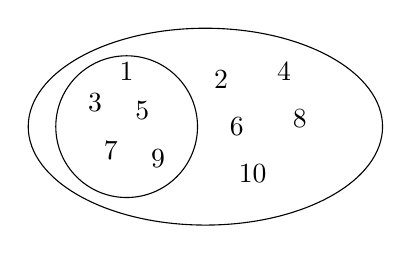
\begin{tikzpicture}
            \draw (0,0) ellipse (2.25 and 1.25);
            \draw (-1,0) circle (0.9);
            \node at (-1,0.7) {$1$};
            \node at (-1.4,0.3) {$3$};
            \node at (-0.8,0.2) {$5$};
            \node at (-1.2,-0.3) {$7$};
            \node at (-0.6,-0.4) {$9$};
            \node at (0.2,0.6) {$2$};
            \node at (1,0.7) {$4$};
            \node at (0.4,0) {$6$};
            \node at (1.2,0.1) {$8$};
            \node at (0.6,-0.6) {$10$};
        \end{tikzpicture}
    %\end{center}
    \item[14.] \hfill\\
        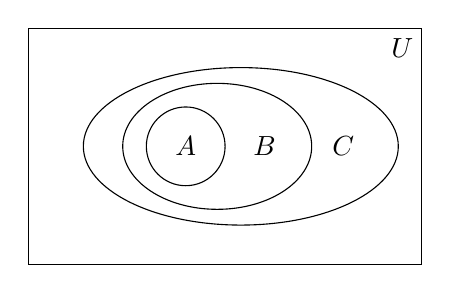
\begin{tikzpicture}
            \draw (0,0) rectangle (5,3);
            \draw (2,1.5) circle (0.5);
            \draw (2.4,1.5) ellipse (1.2 and 0.8);
            \draw (2.7,1.5) ellipse (2 and 1);
            \node at (4.75,2.75) {$U$};
            \node at (2,1.5) {$A$};
            \node at (3,1.5) {$B$};
            \node at (4,1.5) {$C$};
        \end{tikzpicture}
        \qquad where $U$ is the universal set.
    \item[19.]
        \begin{itemize}
            \item[(a)] \fbox{$1$.} The only element is $a$.
            \item[(b)] \fbox{$1$.} The only element is $\{a\}$.
            \item[(c)] \fbox{$2$.} The two elements are $a$ and $\{a\}$.
            \item[(d)] \fbox{$3$.} The three elements are $a$, $\{a\}$, and $\{a, \{ a \} \}$.
        \end{itemize}
    \item[23.]
        \begin{itemize}
            \item[(b)] \fbox{$16$.} $\{ \emptyset, a, \{ a \}, \{ \{ a \} \} \}$ has $4$ elements, so its powerset has $2^4$ elements.
            \item[(c)] \fbox{$2$.} $\mathcal{P}(\mathcal{P}(\emptyset)) = \{ \emptyset, \{ \emptyset \} \}$.
        \end{itemize}
    \item[32.]
        \begin{itemize}
            \item[(a)] $A \times B \times C = \{ (a,x,0), (a,x,1), (a,y,0), (a,y,1),$ \\
            $\phantom{A \times B \times C = \{ } (b,x,0), (b,x,1), (b,y,0), (b,y,1),$ \\
            $\phantom{A \times B \times C = \{ } (c,x,0), (c,x,1), (c,y,0), (c,y,1) \}$
            \item[(b)] $C \times B \times A = \{ (0,x,a), (0,x,b), (0,x,c), (0,y,a), (0,y,b), (0,y,c),$ \\
            $\phantom{C \times B \times A = \{ } (1,x,a), (1,x,b), (1,x,c), (1,y,a), (1,y,b), (1,y,c) \}$
            \item[(c)] $C \times A \times B = \{ (0,a,x), (0,a,y), (0,b,x), (0,b,y), (0,c,x), (0,c,y),$ \\
            $\phantom{C \times A \times B = \{ } (1,a,x), (1,a,y), (1,b,x), (1,b,y), (1,c,x), (1,c,y) \}$
            \item[(d)] $B \times B \times B = \{ (x,x,x), (x,x,y), (x,y,x), (y,x,x),$ \\
            $\phantom{B \times B \times B = \{ } (x,y,y), (y,x,y), (y,y,x), (y,y,y) \}$
        \end{itemize}
    \item[36.] \fbox{$mnp$.} $A \times B \times C$ consists of all ordered triples $(a,b,c)$ where $a \in A$, $b \in B$, and $c \in C$. Since there are $m$ possibilities for $a$, $n$ possibilities for $b$, and $p$ possibilities for $c$, the total number of ordered triples $(a,b,c)$ is the product of $m,n,p$.
    \item[41.]
        \begin{itemize}
            \item[(a)] ``The square of any real number is not $-1$.'' \underline{True.} \\ The square of any real number is nonnegative.
            \item[(d)] ``There exists a real number equal to the square of itself.'' \underline{True.} \\ For example, $0 = 0^2$.
        \end{itemize}
    % 2.2:   2,3,9,12,18(b)(c), 29, 50
    \item[{[\S 2.2]} 2.]
        \begin{itemize}
            \item[(a)] $A \cap B$
            \item[(b)] $A \cap \overline{B}$
            \item[(c)] $A \cup B$
            \item[(d)] $\overline{A \cap B}$ [this is the complement of (a)]
        \end{itemize}
    \item[3.]
        \begin{itemize}
            \item[(a)] $\{ 0,1,2,3,4,5,6 \}$
            \item[(b)] $\{ 3 \}$
            \item[(c)] $\{ 1,2,4,5 \}$
            \item[(d)] $\{ 0,6 \}$
        \end{itemize}
    \item[9.]
        \begin{itemize}
            \item[(a)] $A \cup \overline{A} = \{ x \mid \underbrace{(x \in A) \lor (x \notin A)}_{\textrm{always true}}\} = U$
            \item[(b)] $A \cap \overline{A} = \{ x \mid \underbrace{(x \in A) \land (x \notin A)}_{\textrm{impossible}} \} = \emptyset$
        \end{itemize}
    \item[12.] The other laws in Table~1 can be applied to the left hand side of the equation to show it equals the right hand side:
        \begin{align*}
        A \cup (A \cap B) &= (A \cup A) \cap (A \cup B) \tag*{distributive law} \\
        &= A \cap (A \cup B) \tag*{idempotent law} \\
        &= A \tag*{second absorption law}
        \end{align*}
    \item[18.]
        \begin{itemize}
            \item[(b)] It suffices to show that if $x$ belongs to $(A \cap B \cap C)$ then $x$ also belongs to $(A \cap B)$.

            Suppose $x \in (A \cap B \cap C)$. Then, by definition,
            \[
            (x \in A) \land (x \in B) \land (x \in C),
            \]
            which implies, by simplification,
            \[
            (x \in A) \land (x \in B).
            \]
            Hence $x \in (A \cap B)$. $\square$
            \item[(c)] It suffices to show that if $x$ belongs to $(A-B)-C$ then $x$ also belongs to $A-C$.

            Suppose $x \in (A-B)-C$. Then, by the definition of difference,
            \[
            (x \in A-B) \land (x \notin C).
            \]
            Equivalently, by the same definition,
            \[
            (x \in A) \land (x \notin B) \land (x \notin C),
            \]
            which implies, by simplification,
            \[
            (x \in A) \land (x \notin C).
            \]
            Hence $x \in A-C$. $\square$
        \end{itemize}
    \item[29.]
        \begin{itemize}
            \item[(a)] $B$ is a subset of $A$, since this union implies $B$ contains no elements not in $A$.
            \item[(b)] $A$ is a subset of $B$, since this intersection implies every common element is in $A$.
            \item[(c)] $A$ and $B$ are disjoint, since there was no element in $B$ that existed in $A$.
            \item[(d)] $A$ and $B$ are any two sets. This is an identity (commutative law).
            \item[(e)] $A$ and $B$ are equal. Since
            \begin{align*}
            A - B &= \{ x \in A \mid x \notin B \}, \\
            B - A &= \{ x \in B \mid x \notin A \},
            \end{align*}
            and neither $(x \in A) \land (x \notin A)$ nor $(x \in B) \land (x \notin B)$ is ever possible, both differences result in the empty set;
            \[
            A - B = B - A \quad\Longrightarrow\quad A - B = \emptyset = B - A,
            \]
            which implies every element in $A$ is in $B$, and vice versa.
        \end{itemize}
    \item[50.]
        \begin{itemize}
            \item[(a)] $A_1 = \{ 1, 2, 3, \ldots \}$, $A_2 = \{ 2, 3, 4, \ldots \}$, $A_3 = \{ 3, 4, 5, \ldots \}$, $\ldots$, so the generalized union is $A_1 = \mathbb{Z}^+$ and the generalized intersection is the empty set because no element is common to every set in the collection. \\ %Since $A_1 = \{ 1, 2, 3, 4, \ldots \} = \mathbb{Z}^+ \supset A_2 = \{ 2, 3, 4, \ldots \} = \mathbb{Z}^+ - \{1\} \supset \cdots$ \\
            \fbox{$\displaystyle\bigcup_{i=1}^\infty A_i = \mathbb{Z}^+$ \qquad% \qquad where $\mathbb{Z}^+$ is the set of positive integers \\
            %equivalently $A_1$ since every subsequent set is a subset.
            $\displaystyle\bigcap_{i=1}^\infty A_i = \emptyset$}
            \item[(b)] $A_1 = \{ 0, 1\}$, $A_2 = \{0, 2\}$, $\ldots$, so the generalized union is $\mathbb{N}$, the set of nonnegative integers, and the generalized intersection is $\{ 0\}$ because $0$ is the only number in every set in the collection.\\
            \fbox{$\displaystyle\bigcup_{i=1}^\infty A_i = \mathbb{N}$ \qquad% \qquad where $\mathbb{N}$ is the set of natural numbers including $0$\\
            $\displaystyle\bigcap_{i=1}^\infty A_i = \{ 0 \}$}
            \item[(c)] $A_1 = (0,1)$, $A_2 = (0,2)$, $\ldots$, so the generalized union is $(0,\infty) = \mathbb{R}^+$ and the generalized intersection is $A_1 = (0,1)$ which is the only set that is a subset of every set in the collection.\\
            \fbox{$\displaystyle\bigcup_{i=1}^\infty A_i = \mathbb{R}^+$ \qquad
            $\displaystyle\bigcap_{i=1}^\infty A_i = (0,1)$}
            \item[(d)] $A_1 = (1,\infty)$, $A_2 = (2,\infty)$, $\ldots$, so the generalized union is $A_1 = (1,\infty)$ and the generalized intersection is the empty set because no element is common to every set in the collection.\\
            \fbox{$\displaystyle\bigcup_{i=1}^\infty A_i = (1, \infty)$ \qquad
            $\displaystyle\bigcap_{i=1}^\infty A_i = \emptyset$}
        \end{itemize}
\end{enumerate}
\end{document}